%=====================
\chapter{Requirements}
%=====================
\label{chap:req:requirements}
This chapter describes an \gls{utility} that creates \Gls{wireshark} \glspl{dissector} from \Gls{c}
\gls{header} files. The \glspl{dissector} must interpret \gls{binary} representations of \Gls{c}
\glspl{struct}. In \autoref{sec:req:list} we give a high level overview of the
\gls{utility} and lists all the functional and non-function requirements.

\hyperref[sec:req:stories]{Section \ref*{sec:req:stories}} gives user stories
for the requirements, while \autoref{sec:req:usecases} provides use cases for
the \gls{utility}, and \autoref{sec:prodbacklog} contains the complete product
backlog.

%-----------------------------
\section{List of requirements}
%-----------------------------
\label{sec:req:list}

\subsection{Overview}
%-----------------
We are to create an \gls{utility} that allows \Gls{wireshark} to interpret the \gls{binary}
representations of \Gls{c}-language \glspl{struct}. While \Gls{c} \glspl{struct} seldom are exchanged
across networks, they are sometimes used in \gls{ipc}. The
purpose of the \gls{utility} described here is to provide \Gls{wireshark} with the
capability of automatically dissecting the \gls{binary} representation of a \Gls{c} \gls{struct},
as long as its definition is known.

The expected work flow for the \gls{utility} is to read one or more \Gls{c} \gls{header} files,
which contain \gls{struct} definitions, and output \Gls{wireshark} \glspl{dissector}, implemented
in \Gls{lua} scripts. A configuration file or source code annotations in the \gls{header}
files may be used when additional configuration is required.

\autoref{tab:req:func} lists the functional requirements, while
\autoref{tab:req:nonfunc} lists the non-functional requirements. Each
requirement have a priority (Pri) and a complexity (Cmp): High (H), 
Medium (M) or Low (L) which is explained in \autoref{sec:req:priority} and
\autoref{sec:req:compl}.

\subsection{Prioritization}
%--------------------------
\label{sec:req:priority}
The team has, in cooperation with the customer, prioritized the requirements
in three categories:
\begin{inparaenum}[\itshape a\upshape)]
	\item High,
	\item Medium or
	\item Low.
\end{inparaenum} 

\begin{description}
	\item[High] Core functionality of the \gls{utility} which must be implemented.
	\item[Medium] Requirements that will improve the value of the \gls{utility}.
	\item[Low] Requirements that will not add much value to the \gls{utility}.
\end{description}

\subsection{Complexity}
%----------------------
\label{sec:req:compl}
The team has estimated the complexity for each requirement. We use the same
categories as for requirements priority:
\begin{inparaenum}[\itshape a\upshape)]
	\item High,
	\item Medium or
	\item Low.
\end{inparaenum} 

\begin{description}
	\item[High] Functionality which seems difficult and non-trivial to create.
	\item[Medium] Functionality that seems time consuming but straight forward.
	\item[Low] Requirements that are trivial to implement.
\end{description}

%%%%%%%%%%%%%%%%%%%%%%%%%%%%%%%%%%%%
%%%%%%%%%%%%%%%%%%%%%%%%%%%%%%%%%%%%
%        OBS OBS OBS OBS
%
% These requirements are duplicated
% in many different locations,
% remember to update them all
%
% * product backlog
% * user stories
% * sprint 1 backlog
% * anywhere else?
%
%%%%%%%%%%%%%%%%%%%%%%%%%%%%%%%%%%%%
%%%%%%%%%%%%%%%%%%%%%%%%%%%%%%%%%%%%
\begin{table}[htbp] \footnotesize \center
\caption{Functional Requirements\label{tab:req:func}}
\noindent\makebox[\textwidth]{%
\begin{tabularx}{1.2\textwidth}{l X c c}
	\toprule
	ID & Description & Pri. & Cmp. \\
	\midrule
	FR1 & The \gls{utility} must be able to read basic \Gls{c} language \gls{struct} definitions from \Gls{c} \gls{header} files & H & \\
	FR1-A & The \gls{utility} must support the following basic data types: \gls{int}, \gls{float}, \gls{char} and \gls{boolean} & H & L \\
	FR1-B & The \gls{utility} must support \glspl{member} of type \gls{enum} & H & L \\
	FR1-C & The \gls{utility} must support \glspl{member} of type \gls{struct} & H & M \\
	FR1-D & The \gls{utility} must support \glspl{member} of type \gls{union} & M & M \\
	FR1-E & The \gls{utility} must support \glspl{member} of type \gls{array} & H & M \\
	FR1-F & The \gls{utility} should detect \glspl{struct} with the same name, and report it as an error & M & L \\
	\midrule
	FR2 & The \gls{utility} must be able to generate \Gls{lua} \glspl{dissector} for \Gls{wireshark} for the \gls{binary} representation of \Gls{c} \gls{struct} & H & \\
	FR2-A & The \gls{dissector} shall be able to display simple \glspl{struct} & H & L \\
	FR2-B & The \gls{dissector} shall be able to support \glspl{struct} within \glspl{struct} & M & M \\
	FR2-C & The \gls{dissector} must support \Gls{wireshark}'s built-in filter and search on attributes & H & L \\
	FR2-D & The \gls{dissector} shall be able to recognize invalid values for a \gls{struct} \gls{member} & L & L \\
	\midrule
	FR3 & The \gls{utility} must support \Gls{c} \gls{preprocessor} directives and macros & H & \\
	FR3-A & The \gls{utility} shall support \gls{include} & H & L \\
	FR3-B & The \gls{utility} shall support \\gls{define} and \\gls{if} & H & L \\
	FR3-C & The \gls{utility} shall support \verb+WIN32+, \verb+_WIN32+, \verb+_WIN64+, \verb+__sparc__+, \verb+__sparc+ and \verb+sun+ & M & H \\
	\midrule
	FR4 & The \gls{utility} must support user configuration & M & \\
	FR4-A & Configuration must support valid ranges for \gls{struct} \glspl{member} & L & L \\
	FR4-B & Configuration must support custom \Gls{lua} files for specific \glspl{protocol} & H & H \\
	FR4-C & Configuration must support custom handling of specific data types & L & M \\
	FR4-D & Configuration must support specifying the ID of \glspl{dissector} & H & L \\
	FR4-E & Configuration must support various trailers (other registered \gls{protocol}) & L & H \\
	FR4-F & Configuration must support integer \glspl{member} which represent enumerated named value & M & L \\	
	FR4-G & Configuration must support \glspl{member} which are \gls{bit string} & M & L \\
	\midrule
	FR5 & The \glspl{dissector} must be able to handle \gls{binary} input which size and \gls{endian} depends on originating platform & M & \\
	FR5-A & Flags must be specified in configuration for each platform & M & M \\
	FR5-B & Generate \glspl{dissector} with correct alignment depending on platform & M & M \\
	FR5-C & Generate \glspl{dissector} which support both little and big \gls{endian} platforms & H & M \\
	FR5-D & Generate \glspl{dissector} which support different sizes depending on platforms & M & H \\
	\midrule
	FR6 & The \gls{utility} shall support parameters from command line & H & \\
	FR6-A & Command line shall support parameter for \Gls{c} \gls{header} file & H & L \\
	FR6-B & Command line shall support parameter for configuration file & H & L \\
	FR6-C & Command line shall support batch processing of \Gls{c} \gls{header} and configuration files & L & M \\
	FR6-D & When running \gls{batch mode}, \glspl{dissector} that already are generated, shall not be regenerated, if the source are not modified since last run & L & M \\
	\bottomrule
\end{tabularx}}
\end{table}

\begin{table}[htbp] \footnotesize \center
\caption{Non-Functional Requirements\label{tab:req:nonfunc}}
\noindent\makebox[\textwidth]{%
\begin{tabularx}{1.2\textwidth}{l X c c}
	\toprule
	ID & Description & Pri. & Cmp. \\
	\midrule
	NR1 & The \gls{utility} shall be able to run on latest Windows and \Gls{Solaris} operating system & M & L \\
	\addlinespace
	NR2 & The \gls{dissector} shall be able to run on Windows \gls{x86}, Windows \gls{x86-64}, \Gls{Solaris} \gls{x86}, \Gls{Solaris} \gls{x86-64} and \Gls{Solaris} SPARC & M & M \\
	\addlinespace
	NR3 & The \gls{utility} shall only have a command line user interface. No GUI \& clicking! & H & L \\
	\addlinespace
	NR4 & The \gls{utility} must have sufficient documentation to allow a person, with no previous knowledge of the system or \Gls{wireshark}, to be able to use it to generate \Gls{lua} \glspl{dissector} after 5 hours of reading & M & M \\
	\addlinespace
	NR5 & The \gls{utility} must have sufficient documentation to allow a person, already proficient with the system, to be able to extend its functionality after Y hours of reading & M & M \\
	\addlinespace
	NR6 & The \gls{utility} code should follow standard python coding convention as specified by PEP8 and try to follow python style guidelines defined by PEP20 & H & L \\
	\addlinespace
	NR7 & All Python modules, classes, functions and methods in the \gls{utility} should have docstrings which explains their code & L & L \\
	\bottomrule
\end{tabularx}}
\end{table}


%---------------------
\section{User Stories}
%---------------------
\label{sec:req:stories}
\subsection{Sprint 1}
\label{sec:req:stories1}
This section lists the user stories for the first sprint, these are displayed in \autoref{tab:req:stories1} and \autoref{tab:req:stories2}.
As we are developing a very technical \gls{utility} we have written user stories with an implementation level of abstraction. 
These user stories represent how we intend to add the functionality of the each requirement to the \gls{utility}.
The administrator in this context is the administrator at Thales Norway AS. 
The developer is the person that uses \Gls{wireshark} with the \gls{dissector} generated by CSjark.
This section is subject to change throughout the sprint, as we do not know all the details yet.

\begin{table}[htbp] \footnotesize \center
\caption{User stories - Sprint 1 part 1\label{tab:req:stories1}}
\noindent\makebox[\textwidth]{%
\begin{tabularx}{1.2\textwidth}{l X}
	\toprule
	Header & Value \\
	\midrule
	ID & US01 \\
	Requirements & FR1-A: The \gls{utility} should support the following basic data types: \gls{int}, \gls{float}, \gls{char} and \gls{boolean}. \\
	What & The administrator wants the \gls{utility} to support \glspl{struct} with \glspl{member} of basic data types in input files. 
		These are the basic data types in \Gls{c} which we support: \gls{int}, \gls{float}, \gls{char} and \gls{boolean}.\\
	How & The \Gls{c} \gls{parser} \gls{library}, pycparser, provides this support for us. The input is fed to the cparser module
	which extracts the definitions from an \gls{AST} generated by the \gls{parser}.  \\
	Result & The \gls{utility} supports input with \Gls{c} \glspl{struct} with \gls{int}, \gls{float}, \gls{char} and \gls{boolean} \glspl{member}. \\
	\midrule
	ID & US02 \\
	Requirements & FR2-A: The \gls{utility} shall be able to display simple \glspl{struct}. \\
	What & The developer wants \Gls{wireshark} to display simple \glspl{struct}. \\
	How & The \gls{dissector} module shall generate \Gls{lua} \glspl{dissector} for Protocols created by the cparser module. 
		The \Gls{lua} \glspl{dissector} shall use \Gls{wireshark}'s API to display \glspl{struct} with basic \glspl{member}. \\
	Result & Simple \Gls{c} \glspl{struct} can be dissected in \Gls{wireshark} by our auto generated \Gls{lua} \glspl{dissector}. \\
	\midrule
	ID & US03 \\
	Requirements & FR2-D: Recognize invalid values for a \gls{struct} \gls{member}. \\
	What & The developer wants \Gls{wireshark} to give a warning if a \gls{struct} contains invalid values. \\
	How & The generated \glspl{dissector} contain valid ranges for certain fields, and \Gls{lua} code which adds warning flags 
		in \Gls{wireshark} if a specific fields value is outside the range. \Gls{wireshark} color the display tree yellow to alert the 
		developer of the error. The range is specified by configuration files. \\
	Result & The developer can see when a value is out of range. \\
	\midrule
	ID & US04 \\
	Requirements & FR3-A: The \gls{utility} should support \gls{include}.\\
	What & The administrator wants the \gls{utility} to support the \gls{include}-statement inside a \gls{header} file.\\
	How & The cparser module feeds the input into an external tool, the \Gls{c} \gls{preprocessor}, which supports 
		\gls{include}-statements. It returns a \Gls{c} code file with all the included code from the external files. pycparser
		provides support using a \Gls{c}-\gls{preprocessor}.  \\
	Result & The \gls{utility} supports \gls{include}. \\
	\midrule
	ID & US05 \\
	Requirements & FR3-B: The \gls{utility} should support \gls{define} and \gls{if}. \\
	What & The administrator wants the \gls{utility} to support \gls{define}- and \gls{if}-statement inside a \gls{header} file.\\
	How & The cparser module feeds the input into an external tool, the \Gls{c} \gls{preprocessor}, which supports 
		\gls{define}- and \gls{if}-statements. It returns a copy of the file with the statements removed, and their actions performed. \\
	Result & The \gls{utility} supports \gls{define} and \gls{if} functionality. \\
	\bottomrule
\end{tabularx}}
\end{table}

\begin{table}[htbp] \footnotesize \center
\caption{User stories - Sprint 1 part 2\label{tab:req:stories2}}
\noindent\makebox[\textwidth]{%
\begin{tabularx}{1.2\textwidth}{l X}
	\toprule
	Header & Value \\
	\midrule
	ID & US06 \\
	Requirements & FR4-A: Configuration must support valid ranges for \gls{struct} \glspl{member}. \\
	What & The administrator wants to be able to specify valid ranges for \gls{struct} \glspl{member} in a configuration file. \\
	How & The config module should read config files provided to the command line interface, and find any rules 
		regarding valid ranges. The rules are used by the cparser when it translates \gls{struct} definitions to Protocol 
		and Field instances found in the \gls{dissector} module. \\
	Result & The administrator can specify valid ranges of \gls{struct} \glspl{member} in the configuration.\\
	\midrule
	ID & US07 \\
	Requirements & FR6-A: Command line shall support parameter for \Gls{c}-\gls{header} file. \\
	What & The administrator wants the \gls{utility} to generate a \gls{dissector} from a \Gls{c}-\gls{header} file that he specifies.\\
	How & The command line user interface will accept a number of arguments from the administrator. The 
		argument that includes the path to an existing \Gls{c} \gls{header} file is sent to the \gls{parser} module. The parsing
		of arguments is done with the help of \gls{argparse} \gls{library}, which supports optional and positional arguments etc.\\
	Result & The command line interface supports \Gls{c}-\glspl{header} as input. \\
	\midrule
	ID & US08 \\
	Requirements & FR6-B: Command line shall support parameter for configuration file. \\
	What & The administrator wants to provide the \gls{utility} with one ore more configuration files. \\
	How & The command line interface should accept arguments which specifies the path of existing configuration
		files, and feed these to the config module. The config module should read the files and store them in configuration data 
		structures. These data structures will be available to cparser to help when translating \glspl{struct} to Protocol and
		Fields from the \gls{dissector} module. \\
	Result &  The administrator can input configuration files in the command line.\\
	\bottomrule
\end{tabularx}}
\end{table}

\subsection{Sprint 2}
\label{sec:req:stories2}
This section lists the user stories for the second sprint, these are displayed in \autoref{tab:req:stories3}, \autoref{tab:req:stories4},
\autoref{tab:req:stories5} and \autoref{tab:req:stories6}.
As we are developing a very technical \gls{utility} we have written user stories with an implementation level of abstraction. 
These user stories represent how we intend to add the functionality of the each requirement to the \gls{utility}.
The administrator in this context is the administrator at Thales Norway AS. 
The developer is the person that uses \Gls{wireshark} with the \gls{dissector} generated by CSjark.
This section is subject to change throughout the sprint, as we do not know all the details yet.


\begin{table}[htbp] \footnotesize \center
\caption{User stories - Sprint 2 part 1\label{tab:req:stories3}}
\noindent\makebox[\textwidth]{%
\begin{tabularx}{1.2\textwidth}{l X}
	\toprule
	Header & Value \\
	\midrule
	ID & US09 \\
	Requirement & FR1-B: The \gls{utility} must support \glspl{member} of type \gls{enum} \\
	What & The administrator wants the \gls{utility} to support \glspl{struct} with \glspl{member} of type \gls{enum}. \\
	How & When the cparser module detects an \gls{enum} \gls{member} in a \gls{struct}, the cparser should search in an \gls{enum} dictionary and the \gls{enum} \gls{member} 
		will be mapped to the correct value found in the dictionary. A field representing the \gls{enum} will be added to the prototype object corresponding
		to the enclosing \gls{struct}. \\
	Result & The \gls{utility} supports \glspl{member} of type \gls{enum}. \\
	\midrule
	ID & US10 \\
	Requirement & FR1-C: The \gls{utility} must support \glspl{member} of type \gls{struct} \\
	What & The administrator wants the \gls{utility} to support \glspl{struct} with \glspl{member} of type \gls{struct}. \\
	How & When the cparser module detects a \gls{struct} in the AST that is a \gls{member} of another \gls{struct}, the cparser searches for its definition in the 
		dictionary of previously detected \glspl{struct}. When it finds it, it looks up the identification number and the size of the inner \gls{struct} and creates a 
		struct\_field object with that information inside the prototype object corresponding to the outer \gls{struct}. \\
	Result & The \gls{utility} supports \glspl{member} of type \glspl{struct}. \\
	\midrule
	ID & US11 \\
	Requirement & FR1-F: The \gls{utility} should detect \glspl{struct} with the same name, and report it as an error \\
	What & The administrator wants the \gls{utility} to report an error if it discovers \glspl{struct} with the same name to avoid unforeseen name collisions. \\
	How & When the cparser module traverses the AST to look for \glspl{struct}, it will detect if there are \glspl{struct} with the same name by searching in a database 
		of all \glspl{struct} it has found so far. If a collision is detected the \gls{utility} will crash with an error message. \\
	Result & The \gls{utility} will detect duplicated name of \glspl{struct}. \\
	\midrule
	ID & US12 \\
	Requirement & FR2-B: The \gls{dissector} shall be able to support \glspl{struct} within \glspl{struct} \\
	What & The \gls{utility} should be able to create a \Gls{lua} \gls{dissector} that correctly
	displays \glspl{struct} within \glspl{struct} in \Gls{wireshark}. \\
	How & For each \gls{struct} definition encountered in cparser, a prototype object is created. This object will include an 	identifier number used to locate
		the \Gls{lua} \gls{dissector} for that \gls{struct}. When a \gls{struct} \gls{member} is located inside an outer \gls{struct}. The \gls{dissector} module encodes the identification number 
		and the size for the inner \gls{struct} into the \Gls{lua} \gls{dissector} for the outer \gls{struct}. The identification number is used to access the \gls{dissector} for the inner
		\gls{struct} when the outer \gls{struct} \gls{dissector} is used. The outer \gls{struct} \gls{dissector} uses the size of the inner \gls{struct} to know how much of the network package
		to forward to the inner \gls{struct} \gls{dissector}. The size and identification number of the inner \gls{struct} will be available in the \gls{struct} field corresponding to
		the inner \gls{struct} inside the \gls{protocol} object corresponding to the outer \gls{struct}.  \\
	Result & The \gls{dissector} module supports nested \glspl{struct} \\
	\midrule
	ID & US13 \\
	Requirement & FR4-F: Configuration must support integer \glspl{member} which represent an enumerated named value \\
	What & The administrator wants to specify integer \glspl{member}, represented by an enumerated named value, in a configuration file. \\
	How & The config module should read config files provided to the command line interface, and find any rules regarding enumerated integer values.
		The rules are used by the cparser when it translates 	\gls{struct} definitions to Protocol, and makes the cparser create EnumFields instead of normal
		Fields for the specified \glspl{member}. \\
	Result & Enum \glspl{member} can be specified in the configuration. \\
	\bottomrule
\end{tabularx}}
\end{table}

\begin{table}[htbp] \footnotesize \center
\caption{User stories - Sprint 2 part 2\label{tab:req:stories4}}
\noindent\makebox[\textwidth]{%
\begin{tabularx}{1.2\textwidth}{l X}
	\toprule
	Header & Value \\
	\midrule
	ID & US14 \\
	User doc & FR4-F: User documentation for writing configuration for integer \glspl{member} which represent an enumerated named value. \\
	What & The administrator should be able to educate himself of how to give CSjark the necessary information to get integer values mapped to names in the generated \gls{dissector}. \\
	How & The administrator opens the user documentation and finds the section about configuration. From here he locates the sub section about enumerated names integer values.
	This section gives a good description of how to write such configuration, and the user is able to implement his desired configuration after reading through
	once and looking at provided examples. \\
	Result & The administrator is now able to use the enumerated named value functionality. \\
	\midrule
	ID & US15 \\
	Requirements & FR4-G: Configuration must support \glspl{member} which are \glspl{bit string} \\
	What & The administrator wants to specify \glspl{member} that represent \glspl{bit string} in the configuration. \\
	How & The config module should read config files provided to the command line interface, and find any rules regarding \glspl{bit string}.
	The rules are used by the cparser when it translates \gls{struct} definitions to Protocol and BitField instances found in the \gls{dissector} module. \\
	Result & The administrator can specify \gls{bit string} \glspl{member} in the configuration. \\
	\midrule
	ID & US16 \\
	User doc & FR4-G: User documentation for writing configuration for integer \glspl{member} which are \glspl{bit string}. \\
	What & The administrator should be able to educate himself of how to give CSjark the necessary information to get integer values mapped to \gls{bit string} in 
	the generated \gls{dissector}. \\
	How & The administrator opens the user documentation and finds the section about configuration. From here he locates the sub section about \gls{bit string}
	 integer values. This section gives a good description of how to write such configuration, and the administrator is able to implement his desired configuration
	after reading through once and looking at provided examples.  \\
	Result & The administrator is now able to configure CSjark to generate \gls{dissector} that recognises and formats \glspl{bit string} correctly. \\
	\midrule
	ID & US17 \\
	Requirements & FR1-E: The \gls{utility} must support \glspl{member} of type \gls{array} \\
	What & The administrator wants the \gls{utility} to support \glspl{struct} with \glspl{member} of type \gls{array}. \\
	How & When the cparser module finds an \gls{array} declaration, it recursively traverses the tree until till it encounters the bottom of the declaration 
	to discover the size of the \gls{array}. The \gls{parser} module creates an instance of an \gls{array} field with the size and type of the \gls{array}. From the \gls{array} field
	the \gls{dissector} module generates a \gls{dissector} which has a sub tree for each level of the \gls{array}. \\
	Result & The \gls{utility} support \gls{array} \glspl{member} in \glspl{struct}. \\
	\midrule
	ID & US18 \\
	Requirements & FR4-E: Configuration must support various trailers (other registered \glspl{protocol}) \\
	What & The administrator wants to specify trailers to a \Gls{c} \gls{header} file in the configuration. \\
	How & The config module should read config files provided to the command line interface, and find any rules regarding trailers. A \gls{member} in a \gls{struct}
	will say how many \glspl{packet} of other \glspl{protocol} that follows the \gls{header}. In the config-file it is specified which \gls{member} contains this number, and what
 	type of \gls{protocol} the \gls{packet}(s) belong to. When the \gls{dissector} module generates a \gls{struct} containing a trailer, the correct \gls{dissector} for the trailer \gls{packet}(s) 
	will be called for the rest of the buffer. \\
	Result & The \gls{utility} can handle trailer \glspl{packet} following the \gls{header}, specified in the configuration. \\
	\bottomrule
\end{tabularx}}
\end{table}

\begin{table}[htbp] \footnotesize \center
\caption{User stories - Sprint 2 part 3\label{tab:req:stories5}}
\noindent\makebox[\textwidth]{%
\begin{tabularx}{1.2\textwidth}{l X}
	\toprule
	Header & Value \\
	\midrule
	User doc & FR4-E: User documentation for how to specify trailers (other registered \glspl{protocol}) \\
	What & The administrator should be able to find out how to specify trailers to a \gls{header} \gls{struct} by reading the user documentation. \\
	How & The administrator opens the user documentation and finds the section about configuration. From here he locates the sub section about trailers. 
	This section gives a good description of how to write such configuration for different types of trailers and provides sufficient examples, so that
	it is  clear to the administrator how to write the configuration he needs after reading the section. \\
	Result & The administrator is now able to utilise the trailer feature of CSjark. \\
	\midrule
	ID & US20 \\
	Requirements & FR4-B: Configuration must support custom \Gls{lua} files for specific \glspl{protocol} \\
	What & The administrator wants to specify custom \Gls{lua} files in the configuration, that are to be used in complex cases where our \gls{utility} is unable to generate
	a \gls{dissector} for the \Gls{c} \gls{header}. \\
	How & The config module should read config files provided to the command line interface, and find any rules regarding the use of custom \Gls{lua} files.
	When such a rule is found, the \gls{dissector} module will use the \Gls{lua} code found in the file(s) in addition to its own generated \Gls{lua} code.
	This is done by reading the custom \Gls{lua} file(s) and writing the content to the relevant parts of the \gls{dissector}. \\
	Result & The administrator can specify the use of custom \Gls{lua} file in the configuration. \\
	\midrule
	ID & US21 \\
	Requirements & FR4-C: Configuration must support custom handling of specific types. \\
	What & The administrator will be able to specify that a certain type should be handled in a specific way specified in a configuration file. This configuration must be
 	a \Gls{wireshark} supported lua field. The configuration could both be a global default value for that type, or specific for a \gls{struct} \gls{member}. \\
	How & The config module should read config files provided to the command line interface, and find any rules regarding the use of custom handling of types.
 	It will modify the field added to the prototype field representing the enclosing \gls{struct} with the behaviour specified in the configuration. \\
	Result & The administrator is able to configure custom behaviour for specific types. \\
	\midrule
	ID & US22 \\
	User doc & FR4-C: User documentation for configuring custom handling of specific types. \\
	What & The administrator should be able to find out how to specify custom handling for a specific type by reading the user documentation.\\
	How & The administrator opens the user documentation and finds the section about configuration. From here he locates the sub section about custom type handling. 
	This section gives a good description of how to write such configuration and what kind of configuration that could be done. There should also be some
 	examples to clarify the description. After reading the section, the administrator has a good idea of how to do the desired custom handling. \\
	Result & The administrator is able to use custom handling of specific types. \\
	\midrule
	ID & US23 \\
	Requirements &  FR4-D: Configuration must support specifying the ID of \glspl{dissector} \\
	What & The administrator wants to specify the ID of a \gls{dissector} in a configuration file. \\
	How & When the cparser finds a \gls{struct} in the \gls{AST} it looks for a configuration file for the \gls{struct}. If a config-file is found, the ID of the \gls{dissector}
	is mapped to the ID given in the config-file when generating the \gls{dissector}. \\	
	Result & The administrator can specfiy the ID of \glspl{dissector} in the configuration. \\
	\midrule
	
\end{tabularx}}
\end{table}

\begin{table}[htbp] \footnotesize \center
\caption{User stories - Sprint 2 part 4\label{tab:req:stories6}}
\noindent\makebox[\textwidth]{%
\begin{tabularx}{1.2\textwidth}{l X}
	\toprule
	Header & Value \\
	\midrule
	ID & US24 \\
	Requirements & FR5-C: Generate \glspl{dissector} which support both little and big \gls{endian} platforms \\
	What & The administrator wants the \gls{utility} to produce \glspl{dissector} that can be used on both little and big \gls{endian} platforms. \\
	How & The administrator will specify the platform he is using in a configuration file by adding a message flag and \gls{endian} pair. When the \gls{dissector} for a \gls{struct} is beeng generated,
 	the \gls{dissector} module in CSjark will encode a flag to \gls{endian} dictionary inside the \Gls{lua} \gls{dissector} file. This dictionary will be used to look up the \gls{endian} for a message given 
	its flag. If no \gls{endian} is found in the dictionary, it will use a default value. \\
	Result & The \glspl{dissector} are now able to support messages from platforms with different \gls{endian}. \\
	\midrule
	ID & US25 \\
	Requirements & FR6-C: Command line shall support batch processing of \Gls{c} \gls{header} and configuration files \\
	What & The administrator wants to set up the program to run automatically, so that the program creates \glspl{dissector} from the \Gls{c} \gls{header} and configuration file(s) that are specified. \\
	How & When the administrator feeds the command line with an input argument, \gls{header} or configuration, the \gls{utility} shall check if the input is a single file or a directory (folder). 
	If it is a file, parse it. If it is a folder, retrieve all files in that folder and add them to a list, this list will be sent to the \gls{parser} and all the files will be parsed one after another.
	A directory within a directory should be detected, and traversed recursively. With this approach we can start in a root folder and include all files,
 	independent of the depth. The \gls{batch mode} shall only include files with the extension .h (a \gls{header} file) or .yml (config file), which are the files that are going to be
	parsed as input.   \\
	Result & The administrator can feed the \gls{utility} with folders to make \glspl{dissector} of all the \glspl{header} found, also called \gls{batch mode}. \\
	\bottomrule
\end{tabularx}}
\end{table}

\subsection{Sprint 3}
\label{sec:req:stories3}
This section lists the user stories for the third sprint, these are displayed in \autoref{tab:req:stories7}, \autoref{tab:req:stories8} and \autoref{tab:req:stories9}.
As we are developing a very technical \gls{utility} we have written user stories with an implementation level of abstraction. 
These user stories represent how we intend to add the functionality of the each requirement to the \gls{utility}.
The administrator in this context is the administrator at Thales Norway AS. 
The developer is the person that uses \Gls{wireshark} with the \gls{dissector} generated by CSjark.
This section is subject to change throughout the sprint, as we do not know all the details yet.


\begin{table}[htbp] \footnotesize \center
\caption{User stories - Sprint 3 part 1\label{tab:req:stories7}}
\noindent\makebox[\textwidth]{%
\begin{tabularx}{1.2\textwidth}{l X}
	\toprule
	Header & Value \\
	\midrule
	ID & US26 \\
	Requirement & FR1-D: The \gls{utility} must support \glspl{member} of type \gls{union} \\
	What & The administrator wants to generate \glspl{dissector} which contain \glspl{struct} with unions as \glspl{member}. \\
	How & When the administrator feeds the \gls{utility} with a \gls{header} containing a \gls{union}, the cparser module should parse the \gls{union} and its \glspl{member} to find the total size of the 
	\gls{union} (which equals the size of the largest \gls{member}), and then create an instance of UnionField from the \gls{dissector} module representing the \gls{union} and its \gls{member}\\
	Result & The \gls{utility} support \gls{union} \glspl{member} in \glspl{struct}. \\
	\midrule
	ID & US27 \\
	Requirements & FR2-A\textit{Addition:} Display a \gls{wildcard} type for valid \Gls{c} types that \Gls{wireshark} has no support for. \\
	What & The administrator should be able to give the tool a \gls{struct} with a valid \Gls{c}-type even if \Gls{wireshark} does not have a way to display that type in a natural way.
	The \gls{dissector} should the just display the name of the type, the name of the \gls{member} and the hex value from the \gls{packet}. \\
	How & The \gls{parser} module will recognise if a type it encounters are supported in \Gls{wireshark} or not. If it is not supported, it will add a \gls{wildcard} field to the prototype object
	representing the enclosing \gls{struct}. \\
	Result & The administrator will be able to both run the \gls{utility} and get some information from the \gls{dissector} even if the type used is not supported by \Gls{wireshark}. \\
	\midrule
	ID & US28 \\
	Requirements & FR2-C: Filter and search on attributes (important to have descriptive abbreviations) \\
	What & The developer wants to find specific attributes in \Gls{wireshark}. The amount of data captured can be big.
	After the \glspl{packet} have been dissected, they are presented in \Gls{wireshark}. The developer will have a hard time finding 
	attributes by manual seeking. The built-in search and filter functionality needs to be supported to accommodate the developer. \\
	How & The functionality is already in \Gls{wireshark}. To utilize it, an abbreviation field must be provided to \Gls{wireshark}. This abbreviation field will be in the \gls{dissector} module
	and is included in the \gls{dissector} generated by the \gls{utility}. When \Gls{wireshark} runs the \gls{dissector}, all abbreviations are collected which will make it possible to filter and search
	on attributes. \\
	Result & The developer will be able to search and filter by attributes. \\
	\midrule
	ID & US29 \\
	Requirements & FR5-A: Flags must be specified in configuration for each platform \\
	What & The administrator wants to generate \glspl{dissector} which are different depending on platform. \\
	How & To be able to create \glspl{dissector} which are different depending on the originating platform, the administrator needs to specify in the configuration which platforms he wants to support.
	The config module should accept such configuration and store it so other modules can use it. \\ 
	Result & The administrator can specify what platform he is using by setting a flag in the configuration. \\
	\midrule
\end{tabularx}}
\end{table}

\begin{table}[htbp] \footnotesize \center
\caption{User stories - Sprint 3 part 2\label{tab:req:stories8}}
\noindent\makebox[\textwidth]{%
\begin{tabularx}{1.2\textwidth}{l X}
	\toprule
	Header & Value \\
	\midrule
	ID & US31 \\
	Requirement & FR5-C: Generate \glspl{dissector} which support both little and big \gls{endian} platforms \\
	What & The administrator wants \glspl{dissector} which handle both big and little \gls{endian} encoding. \\
	How & The \gls{dissector} module will need to create different lua code for big and little \gls{endian}, when adding nodes to the \Gls{wireshark} tree and when calling other \glspl{dissector}.
	The \gls{dissector} module shall have functionality which generates lua code depending on \gls{endianness}, and the different Field classes must use this function when adding 
	nodes to the \Gls{wireshark} tree. \\
	Result & Dissectors can be created with platform specific \gls{endian}. \\
	\midrule
	ID & US32 \\
	Requirements & FR5-D: Generate \glspl{dissector} which support different sizes depending on platforms \\
	What & The administrator wants to generate \glspl{dissector} for \gls{struct} where \glspl{member} size depend on the originating platform. \\
	How & When the administrator feeds the \gls{utility} a \gls{header} file and a config file with a set of platform he wants \glspl{dissector} for, the config module will create new \gls{header} files
	with \Gls{c} \gls{preprocessor} directives for each platform. These files should define platform-specific macros which emulates parsing on the specific platform. 
	The \gls{dissector} module then create different \glspl{dissector} for each message on each platform, and a mapping is added inside the master \Gls{lua} file which maps message id and
	platform to the correct \gls{dissector}. \\
	Result & Dissectors can be created with platform specific sizes of \glspl{member}.\\
	\midrule
	ID & US33 \\
	Requirements & FR3-C: Support for configuring a platform with a platform specific macro like WIN32, \_WIN64, \_\_sparc to be able to  support different \gls{struct} definitions 
	for different platforms. \\
	What & The administratorwants to be able to configure the \gls{utility} to make \glspl{dissector} that support \glspl{struct} that is defined differently on different platforms via platform specific
	macros like WIN32, \_WIN64, \_\_sparc. \\
	How & The administrator specify the macro associated with a platform together with the platform definition configuration. The \gls{utility} then make an auxiliary \gls{header} file for each 
	platform configuration with the specified macro definition. These \glspl{header} are forwarded to the \gls{parser} module, which uses them to generate
  	one \gls{dissector} for each platform for each \gls{struct}. All \glspl{dissector} dissecting the same \glspl{struct} are stored in the same file, but are added to a platform specific \gls{dissector} table. \\
	Result & The generated \Gls{lua} files corresponding to \glspl{struct} now includes one \gls{dissector} for each platform defined in the configuration file. \\
	\midrule
	ID & US34 \\
	User doc & FR4-C: User documentation for configurating custom handling of specific types. \\
	What & The administrator should be able to find out how to specify custom handling for a specific type by reading the user documentation. \\
	How &	 The administrator opens the user documentation and finds the section about configuration. From here he locates the sub section about custom type handling. 
	This section gives a good description of how to write such configuration and what kind of configuration that could be done. There should also be some examples to clarify
	the description. After reading the section, the user has a good idea of how to do the desired custom handling. \\ 
	Result & The administrator is able to use custom handling of specific types. \\
	\midrule

\end{tabularx}}
\end{table}

\begin{table}[htbp] \footnotesize \center
\caption{User stories - Sprint 3 part 3\label{tab:req:stories9}}
\noindent\makebox[\textwidth]{%
\begin{tabularx}{1.2\textwidth}{l X}
	\toprule
	Header & Value \\
	\midrule
	ID & US35 \\
	Requirements & FR4-D modified: Configuration must support specifying the ID of \glspl{dissector} \\
	What & The administrator wants to specify the ID of a \gls{dissector} in a configuration file. The \glspl{dissector} should not be given any ID if it has not been specifically configured. \\
	How & When the cparser finds a \gls{struct} in the \gls{AST} it looks for a configuration file for the \gls{struct}. If a config-file is found, the	ID of the prototype field
	representing the \gls{dissector} will be mapped to the ID given in the config-file.  If it is not found, the ID will be sat to NONE. \\
	Result & The administrator can specify the ID of \glspl{dissector} in the configuration. \\
	\midrule
	ID & US36 \\
	User doc & FR5 User documentation for how to add or remove support for a platform in the \glspl{dissector} generated from the \glspl{utility}. \\
	What & The administrator should be able to find out how to add or remove support for a platform in the \glspl{dissector} by reading the user documentation. \\
	How & The administrator opens the user documentation and finds the section about configuration. From here he locates the sub section about platform support. 
	This section gives a good description of how to add or remove support for a platform in the configuration, so that the administrator understands how to do
	this after reading the section. \\
	Result & The administrator is now able to configure the \gls{utility} to add or remove platform support from the generated \glspl{dissector}. \\
	\midrule
	ID & US37 \\
	User doc & FR5 User documentation for what platform that the \gls{utility} support. \\
	What & The administrator should be able to find out what platforms he can add support for in the custom \gls{dissector} files. \\
	How & The administrator opens the user documentation and finds the section about configuration. From here he locates the sub section about platform support.
	This section gives a list of currently supported platforms by the \gls{utility}. It should also have some information of where to	find the documentation that describes
	how to add support for more platforms. \\
	Result & The administrator is now able to look up what platforms he can get the \glspl{dissector} to support. \\
	\midrule
	ID & US38 \\
	Requirements & FR6-D The \gls{utility} should not regenerate \glspl{dissector} within a single run. \\
	What & The administrator should be able to specify folder that includes both a standalone \gls{header} file with a \gls{struct} definitions and another \gls{header} file that includes
	the first \gls{header}. The \gls{utility} will only generate the \gls{dissector} once for the \gls{struct} inside the first \gls{header}. \\
	How & For each \gls{struct} encountered, the \gls{utility} will check the table of generated \glspl{dissector} to see if there is an existing \gls{dissector} generated for the \gls{struct} name.
	It will only generate a new \gls{dissector} if the table of \glspl{dissector} is empty for that name. \\
	Result & The \gls{utility} will run faster as a result of not needing to regenerate \glspl{dissector}. \\
	\midrule
	ID & US39 \\
	Requirements & Handle \Gls{lua} reserved definition names \\
	What & The \Gls{c} \glspl{struct} could contain \glspl{member} with names that are reserved by \Gls{lua}. The \gls{dissector} module needs to avoid creating \Gls{lua} variables with such names.  \\
	How &	 The \gls{dissector} module has a method called create\_lua\_var. This method will ensure that variable names are valid, by comparing the variable names to a list
	of \Gls{lua} reserved keywords, and if there is a match we need to add an underscore in front of the variable name. \\ 
	Result & The \gls{utility} can handle \Gls{c} \gls{header} files that contain \Gls{lua} reserved definition names. \\
	\bottomrule
\end{tabularx}}
\end{table}

%------------------
\section{Use Cases}
%------------------
\label{sec:req:usecases}
This sections contains use case diagrams for our two actors, and detailed
textual use cases for these diagrams.

\subsection{Actors}
%------------------
An actor specifies a role played by an external person or thing that interact
with our \gls{utility}. We have three types of actors to consider. First is the
primary actor which in our case is the user of our \gls{utility}. He who feeds it a
\Gls{c} file to generate \glspl{dissector}. A secondary actor is someone who configures our
\gls{utility} to change the output of it. Finally we have an offstage actor which
does not use our \gls{utility} himself, but uses the output \glspl{dissector} in \Gls{wireshark}.

We have defined two use case actors for our \gls{utility}. The customer has specified
that the offstage actor, called administrator, is the most important actor.
\begin{description}
	\item[Developer] User of the generated \Gls{wireshark} \glspl{dissector}, offstage actor
	\item[Administrator] User and configurer of \gls{utility}, primary and secondary actor
\end{description}

\subsection{Use Case Diagrams}
%-----------------------------
\hyperref[fig:req:ucadm]{Figure \ref*{fig:req:ucadm}} shows the use case
diagram for the administrator, and \autoref{fig:req:ucdev} is the use case
diagram for the developer.
\begin{figure}[htbp]
	\center
	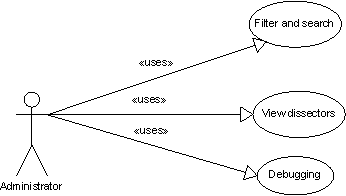
\includegraphics[width=0.8\textwidth]{./planning/img/administrator}
	\caption{Use Case Diagram: Administrator\label{fig:req:ucadm}}
\end{figure}

\begin{figure}[htbp]
	\center
	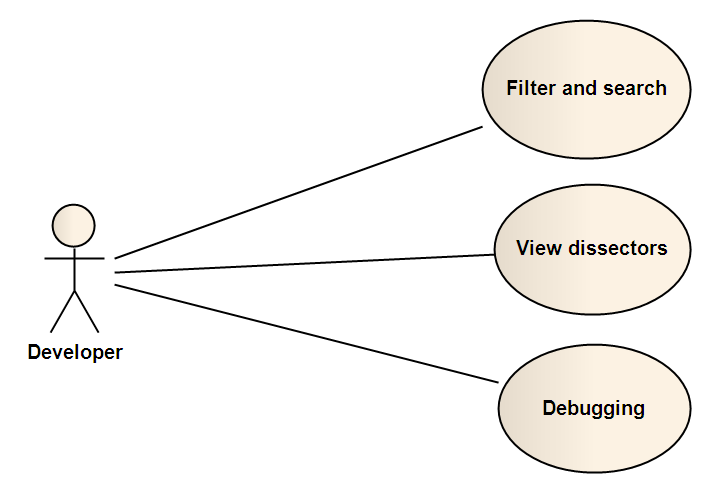
\includegraphics[width=0.8\textwidth]{./planning/img/developer}
	\caption{Use Case Diagram: Developer\label{fig:req:ucdev}}
\end{figure}

%Removed for pre-delivery
%\subsection{Textual Use Cases}
%-----------------------------
%TODO!!!

